\documentclass{beamer}
\usepackage{graphics}
\usepackage{epsfig}
\usepackage{multicol}
\usepackage{pifont}
\setbeamertemplate{navigation symbols}{}

\newcommand{\RR}{\ensuremath{\mathbb{R}}}
\newcommand{\NN}{\ensuremath{\mathbb{N}}}
\newcommand{\QQ}{\ensuremath{\mathbb{Q}}}
\newcommand{\CC}{\ensuremath{\mathbb{C}}}
\newcommand{\ZZ}{\ensuremath{\mathbb{Z}}}
\newcommand{\TT}{\ensuremath{\mathbb{T}}}
\DeclareMathOperator{\Min}{Min}
\DeclareMathOperator{\Dom}{Dom}
\DeclareMathOperator{\vol}{vol}
\DeclareMathOperator{\Aut}{Aut}
\DeclareMathOperator{\Stab}{Stab}
\DeclareMathOperator{\Sym}{Sym}
\DeclareMathOperator{\Grp}{Grp}
\DeclareMathOperator{\GL}{GL}
\DeclareMathOperator{\Id}{Id}

\begin{document}
\title{Space fullerenes}
\author{
{\small
\begin{multicols}{2}
\textcolor{red}{\large Olaf Delgado Friedrichs}\\[2mm]
\textcolor{red}{The Australian National University, Canberra}\\[2mm]
\textcolor{red}{\large Michel Deza}\\[2mm]
\textcolor{red}{Institut Statistical Mathematics, Tokyo}
\end{multicols}
\begin{center}
\textcolor{red}{\large Mathieu Dutour Sikiri\'c}\\[2mm]
\textcolor{red}{Institut Rudjer Boskovic, Zagreb}
\end{center}
}
}
\date{\today} 

\frame{\titlepage} 

%\frame{\frametitle{Table of contents}\tableofcontents} 
%
%\section{Section 1}


%\frame{
%\begin{center}
%\begin{tabular*}{7cm}{c}
%\\[-0.5cm]
%{\Huge
%\textcolor{blue}{I. }\textcolor{red}{Fullerenes}
%}
%\end{tabular*}
%\end{center}
%}




%\frame{
%  \frametitle{Generation of plane graphs}
%\begin{itemize}
%\item There exist now several different algorithms and programs for generating plane graphs
%\item {\tt \textcolor{red}{plantri}} (by Brendan McKay and Gunnar Brinkmann): This program can generates with optimal speed:
%\begin{itemize}
%\item Triangulations of the sphere,
%\item Triangulations of the sphere of minimum degree $4$ or $5$,
%\item Eulerian triangulations of the sphere,
%\item Quadrangulation of the sphere,
%\item $3$-connected plane graphs,
%\item plane graphs, 
%\item $3$-connected plane graphs of minimum degree at least $4$ or $5$.
%\end{itemize}
%All this is done using the canonical path method.
%\item {\tt \textcolor{red}{FullGen CPF, \& ENU}} (by Gunnar Brinkmann and Thomas Harmuth), they can generate $3$- or $4$-valent plane graphs such that the number of faces of size $a$ is fixed equal to $p_a$.\\
%\item The method is to use zigzags and central circuits:
%\begin{center}
%\begin{minipage}[t]{7cm}
%\centering
%\epsfig{file=CanadaPicture/Tight88_Tsec.pdf, height=3cm}\par
%Simple zigzag in a $88$-vertex\\
%$3$-valent plane graph.
%\end{minipage}
%\begin{minipage}[t]{7cm}
%\centering
%\epsfig{file=CanadaPicture/oc30-1thi.pdf, height=3cm}\par
%Simple central circuit in a $30$-vertex\\
%$4$-valent plane graph.
%\end{minipage}
%\end{center}
%\item If the zigzag or central circuit is simple, then:
%\begin{itemize}
%\item We enumerate the fillings on either side,
%\item We glue them in all possible ways,
%\item We reduce by isomorphism and obtain all possible fillings.
%\end{itemize}
%If the circuits are not simple, then there is still a way (more complicate).
%\item {\tt \textcolor{red}{CGF}} (by Thomas Harmuth): It generates $3$-valent orientable maps on 
%\end{itemize}
%}


%\frame{
%  \frametitle{Drawing graphs}
%
%\begin{itemize}
%\item Plane graph drawing is done using an algorithm of Tutte implemented in {\tt \textcolor{red}{CaGe}}.
%\begin{itemize}
%\item[\textcolor{red}{\ding{224}}] G. Brinkmann, O. Delgado Friedrichs, A. Dress and T. Harmuth, {\em CaGe -- a virtual environment for studying some special classes of large molecules}, MATCH: Communications in Mathematical and in Computer Chemistry, {\bf 36} (1997) 233--237.
%\end{itemize}
%\item 
%
%\end{itemize}
%}


%\frame{
%  \frametitle{Circle packing methods}
%
%\begin{itemize}
%\item A map $G$ is called \textcolor{blue}{reduced} if its universal cover is $3$-connected.
%\item Given a reduced map $G$, we can find
%in polynomial time an embedding of $G$ on a surface $S$ of constant
%curvature such that
%\begin{itemize}
%\item Every vertex $v$ has a circle $C_v$
%\item Two circles $C_v$ and $C_{v'}$ share a vertex if and only if $v$ and $v'$ are adjacent.
%\item Every face $F$ has a circle $C_F$
%\item Two circles $C_F$ and $C_{F'}$ share a vertex if and only if $F$ and $F'$ are adjacent.
%\item if an edge contains 
%\end{itemize}
%\item Getting those circle radius is done in a polynomial time, with a reasonable algorithm.
%\begin{itemize}
%\item[\textcolor{red}{\ding{224}}] B. Mohar, {\em Circle packing of map in polynomial time}, European Journal of Combinatorics {\bf 18} (1997) 785--805.
%\end{itemize}
%\end{itemize}
%}

\frame{
\begin{center}
\begin{tabular*}{7cm}{c}
\\[-0.5cm]
{\Huge
\textcolor{blue}{I. }\textcolor{red}{Space fullerenes}
}
\end{tabular*}
\end{center}
}


\frame{
  \frametitle{Fullerenes}

\begin{itemize}
\item A fullerene is a $3$-valent plane graph, whose faces are $5$ or $6$-gonal.
\item They exist for any even $n\geq 20$, $n\not= 22$.
\begin{center}
%\begin{minipage}[b]{2.3cm}
%\centering
%\resizebox{20mm}{!}{\includegraphics[bb=1 1 440 381, clip]{PictureAppli/F2sec.pdf}}\par
%24
%\end{minipage}
%\begin{minipage}[b]{2.3cm}
%\centering
%\resizebox{20mm}{!}{\includegraphics[bb=1 1 457 464, clip]{FullPresPic/Picture2.pdf}}\par
%26
%\end{minipage}
\begin{minipage}[b]{2.3cm}
\centering
\resizebox{13mm}{!}{\rotatebox{90}{\includegraphics[bb=1 1 333 395, clip]{FullPresPic/Picture3.pdf}}}\par
\end{minipage}
%\begin{minipage}[b]{2.3cm}
%\centering
%\resizebox{20mm}{!}{\includegraphics[bb=1 1 439 380, clip]{PictureAppli/F4sec.pdf}}\par
%28
%\end{minipage}
\begin{minipage}[b]{2.3cm}
\centering
\resizebox{11mm}{!}{\includegraphics[bb=1 1 377 398, clip]{FullPresPic/Picture5.pdf}}\par
\end{minipage}
\begin{minipage}[b]{2.3cm}
\centering
\resizebox{13mm}{!}{\includegraphics[bb=1 1 429 374, clip]{FullPresPic/Picture6.pdf}}\par
\end{minipage}
\begin{minipage}[b]{2.3cm}
\centering
\resizebox{13mm}{!}{\includegraphics[bb=1 1 385 335, clip]{FullPresPic/Picture7.pdf}}\par
\end{minipage}
\end{center}
\item There exist extremely efficient programs to enumerate them (\textcolor{red}{FullGen} by G. Brinkman, \textcolor{red}{CPF} by T. Harmuth)
\item Fullerenes with isolated pentagons have $n\geq 60$. The smallest one:
\begin{center}
\begin{minipage}{4.5cm}
\centering
\resizebox{30mm}{!}{\includegraphics[bb=26 165 568 678, clip]{DRAW/PS/C60.pdf}}\par
\end{minipage}
\begin{minipage}{4.5cm}
\centering
{\em Truncated icosahedron},\par
{\em soccer ball},\par
{\em Buckminsterfullerene}
\end{minipage}


\end{center}
\end{itemize}
}


\frame{
  \frametitle{Frank Kasper structures}

\begin{itemize}
\item There are exactly $4$ fullerenes with isolated hexagons:
\begin{center}
\begin{minipage}[b]{24mm}
\centering
\resizebox{18mm}{!}{\rotatebox{90}{\includegraphics[bb=86 165 524 626,clip]{SpaceFullPicture/F1.pdf}}}\par
20
\end{minipage}
\begin{minipage}[b]{24mm}
\centering
\resizebox{20mm}{!}{\includegraphics[bb=1 1 440 381, clip]{PictureAppli/F2sec.pdf}}\par
%\resizebox{18mm}{!}{\rotatebox{0}{\includegraphics[bb=86 206 524 590,clip]{SpaceFullPicture/F2.pdf}}}\par
24
\end{minipage}
\begin{minipage}[b]{24mm}
\centering
\resizebox{20mm}{!}{\includegraphics[bb=1 1 457 464, clip]{FullPresPic/Picture2.pdf}}\par
%\resizebox{18mm}{!}{\rotatebox{0}{\includegraphics[bb=86 206 524 590,clip]{SpaceFullPicture/F3.pdf}}}\par
26
\end{minipage}
\begin{minipage}[b]{24mm}
\centering
\resizebox{20mm}{!}{\includegraphics[bb=1 1 439 380, clip]{PictureAppli/F4sec.pdf}}\par
%\resizebox{18mm}{!}{\rotatebox{0}{\includegraphics[bb=86 206 524 590,clip]{SpaceFullPicture/F4.pdf}}}\par
28
\end{minipage}
\end{center}
\item A \textcolor{red}{Space-fullerene} structure is a $4$-valent $3$-periodic tiling of $\RR^3$ by those $4$ fullerenes.
\item They occur in:
\begin{itemize}
\item ordered tetrahedrally closed-packed phases of metallic
alloys with cells being atoms. There are $>20$ t.c.p. alloys named \textcolor{red}{Frank-Kasper} structures.
\item soap froths (foams, liquid crystals)
\item hypothetical silicate (or zeolite) if vertices are
tetrahedra $SiO_4$ (or $SiAlO_4$) and cells $H_2O$
\item better solution to the Kelvin problem
\end{itemize}


\end{itemize}
}


\frame{
  \frametitle{Main examples of space fullerenes}
Also in clathrate ``ice-like'' hydrates: vertices are
$H_2O$, hydrogen bonds, cells are sites of solutes
($Cl$, $Br$, \dots). 

{\scriptsize
\begin{center}
\begin{tabular}{|c|c|c|c|c|c|c|}
\hline
t.c.p.   & alloys  & exp. clathrate  &\# $20$&\# $24$&\# $26$&\# $28$\\
\hline
$A_{15}$ &$Cr_{3}.Si$  & I:$4Cl_2.7H_2O$       &1  &3 &0 &0\\
$C_{15}$ &$MgCu_2$     & II:$CHCl_3.17H_2O$    &2  &0 &0 &1\\
$Z$      &$Zr_4Al_3$   & III:$Br_2.86H_2O$     &3  &2 &2 &0\\
$\sigma$ &$Cr_{46}.Fe_{54}$ &                  &5  &8 &2 &0\\
$\mu$    &$Mo_6Co_7$   &                       &7  &2 &2 &2\\
$\delta$ &$MoNi$       &                       &6  &5 &2 &1\\
$C$      &$V_2(Co,Si)_3$&                      &15 &2 &2 &6\\
$T$      &$Mg_{32}(Zn,Al)_{49}$& $T_I$ (Bergman)&49 &6 &6 &20\\
$SM$     &             &$T_P$ (Sadoc-Mossieri)  &49 &9 &0 &26\\
\hline
\end{tabular}
\end{center}
}
\begin{itemize}
\item J.M. Sullivan, {\em New tetrahedrally closed-packed structures}.
\end{itemize}
}



%\frame{
%  \frametitle{Frank-Kasper polyhedra and $A_{15}$}

%\begin{center}
%\begin{minipage}{5.5cm}
%\centering
%\resizebox{5cm}{!}{\includegraphics[bb=176 30 420 267, clip]{PictureAppli/fig14.eps}}\par
%\end{minipage}
%\end{center}

%Mean face-size of all known space fullerenes is in $[5 + \frac{1}{10} (C_{15}), 5 + \frac{1}{9} (A_{15})]$.
%Closer to impossible $5$ ($120$-cell on $3$-sphere) means energetically competitive with diamond.
%
%}



\frame{
  \frametitle{A special tiling by fullerenes}
There exist tilings by fullerenes different from $F_{20}$, $F_{24}$,
$F_{26}$ and $F_{28}(T_d)$.
By $F_{20}$, $F_{24}$ and its elongation $F_{36}(D_{6h})$
in ratio $7:2:1$;

\begin{center}
\begin{minipage}[b]{5.0cm}
\centering
\resizebox{4.1cm}{!}{\includegraphics[bb=1 4 434 485, clip]{FullPresPic/Scrn1s.pdf}}\par
\end{minipage}
\begin{minipage}[b]{5.0cm}
\centering
\resizebox{4.1cm}{!}{\includegraphics[bb=3 3 511 595, clip]{FullPresPic/Scrn3s.pdf}}\par
\end{minipage}
\end{center}
\begin{itemize}
\item All tiling by fullerenes with at most $7$ kinds of flags:\par
$A_{15}$, $C_{15}$, $Z$, $\sigma$ and this one (by Deza and Shtogrin).
(Delgado, O'Keeffe).
\end{itemize}
}




\frame{
  \frametitle{Kelvin problem}
Partition $E^3$ into cells of equal volume and minimal surface.

\begin{center}
\begin{minipage}[b]{5.0cm}
\centering
\resizebox{4.0cm}{!}{\includegraphics[bb=10 22 278 265, clip]{FullPresPic/kelvinend_4.pdf}}\par
Kelvin's partition
\end{minipage}
\begin{minipage}[b]{5.0cm}
\centering
\resizebox{3.5cm}{!}{\includegraphics[bb=36 15 250 277, clip]{FullPresPic/wpC_4.pdf}}\par
Weaire, Phelan's partition
\end{minipage}
\end{center}
\begin{itemize}
\item Weaire-Phelan partition ($A_{15}$) is 0.3\% better than Kelvin's, best is unknown 
\item In dimension $2$, best is honeycomb (Ferguson, Hales)
\end{itemize}
}





\frame{
\begin{center}
\begin{tabular*}{7cm}{c}
\\[-0.5cm]
{\Huge \textcolor{blue}{II. }\textcolor{red}{Combinatorial}}\\
{\Huge \textcolor{red}{encoding and}}\\
{\Huge \textcolor{red}{topological recognition}}\\
{\Huge \textcolor{red}{problem}}
\end{tabular*}
\end{center}
}


\frame{
  \frametitle{Flags and flag operators}

\begin{itemize}
\item A \textcolor{red}{cell complex} ${\cal C}$ is a family of cells with inclusion relations such that the intersection of any two cells is either empty or a single cell.\\
We also assume it to be pure of dimension $d$, i.e. all inclusion maximal cell have dimension $d$.
\item It is \textcolor{red}{closed} (or has \textcolor{red}{no boundary})
if any $d-1$ dimensional cell is contained in two $d$-dimensional cells.
\item A \textcolor{red}{flag} is an increasing sequence $F_{n_0}\subset F_{n_1}\subset \dots \subset F_{n_r}$ of cells of dimension $n_0,\dots, n_r$. $(n_0,\dots, n_r)$ is the type of the flag.
\item A flag is \textcolor{red}{complete} if its type is $(0,\dots, d)$.
\item Denote by ${\cal F}({\cal C})$ the set of complete flags of ${\cal C}$.
\item If $f=(F_0,\dots, F_d)$ is a complete flag and $0\leq i\leq d$ then the flag $\sigma_i(f)$ is the one differing from $f$ only in the dimension $i$.
\item A cell complex ${\cal C}$ is completely described by the action of $\sigma_i$ on ${\cal F}({\cal C})$.
\item The problem is that ${\cal F}({\cal C})$ may well be infinite or very large to be workable with.
\end{itemize}
}



\frame{
  \frametitle{Delaney symbol}

\begin{itemize}
\item Suppose ${\cal C}$ is a cell complex, with a group $G$ acting on it. The \textcolor{red}{Delaney symbol} of ${\cal C}$ with respect to $G$ is a combinatorial object containing:
\begin{itemize}
\item The orbits $O_k$ of complete flags under $G$
\item The action of $\sigma_i$ on those orbits for $0\leq i\leq d$.
\item For every orbit $O_k$, take $f\in O_k$, the smallest $m$ such that $(\sigma_i\sigma_j)^m(f)=f$ is independent of $f$ and denoted $m_{i,j}(k)$.
\end{itemize}
${\cal C}$ quotiented by $G$ is an \textcolor{red}{orbifold}.
\item If $G=\Aut({\cal C})$ we speak simply of \textcolor{red}{Delaney symbol} of ${\cal C}$
\item \textcolor{blue}{Theorem}: If ${\cal C}$ is a simply connected manifold, then it is entirely described by its Delaney symbol.
\begin{itemize}
\item A.W.M. Dress, {\em Presentations of discrete groups, acting on simply connected manifolds, in terms of parametrized systems of Coxeter matrices---a systematic approach}, Advances in Mathematics {\bf 63-2} (1987) 196--212.
\end{itemize}
\end{itemize}
}


\frame{
  \frametitle{The inverse recognition problem}

\begin{itemize}
\item Suppose we have a Delaney symbol ${\cal D}$, i.e. the data of permutations $(\sigma_i)_{0\leq i\leq d}$ and the matrices $m_{ij}(k)$.
\begin{center}
\begin{tabular}{p{8cm}}
We want to know what is the universal cover manifold ${\cal C}$ (and if it is Euclidean space).
\end{tabular}
\end{center}
\item Some cases:
\begin{itemize}
\item If we have only \textcolor{red}{$1$ orbit of flag} then the Delaney symbol is simply a Coxeter Dynkin diagram and the decision problem is related to the eigenvalues of the Coxeter matrix.
\item If \textcolor{red}{$d=2$} then we can associate a curvature $c({\cal D})$ to the Delaney symbol and the sign determines whether ${\cal C}$ is a sphere, euclidean plane or hyperbolic plane.
\item If \textcolor{red}{$d=3$} then the problem is related to hard questions in $3$-dimensional topology. But the software Gavrog/3dt by Olaf Delgado can actually decide those questions.
\end{itemize}

\end{itemize}
}


\frame{
  \frametitle{Functionalities of Gavrog/3dt}


\begin{itemize}
\item It can
\begin{itemize}
\item Test for euclidicity of Delaney symbols, that is recognize when ${\cal C}$ is Euclidean space.
\item Find the minimal Delaney symbol, i.e. the representation with smallest fundamental domain and maximal group of symmetry.
\item Compute the space group of the crystallographic structure.
\item Test for isomorphism amongst minimal Delaney symbols.
\item Create pictures, i.e. metric informations from Delaney symbols.
\end{itemize}
\item All this depends on difficult questions of $3$-dimensional topology, some unsolved.
This means that in theory the program does not always works, but in practice it does.
\begin{itemize}
\item[\textcolor{red}{\ding{224}}] O. Delgado Friedrichs, {\em 3dt - Systre},
\begin{center}
\url{http://gavrog.sourceforge.net}
\end{center}
\item[\textcolor{red}{\ding{224}}] O. Delgado Friedrichs, {\em Euclidicity criteria}, PhD thesis.
\end{itemize}

\end{itemize}
}



%\frame{
%  \frametitle{Enumeration strategies}
%\begin{itemize}
%\item In all cases, it is a two steps procedure:
%\begin{itemize}
%\item Enumerate the combinatorial types sought (time and memory limited, but conceptually simple).
%\item Test Euclidicity and represent the structures (very sophisticated method, but not the blocking part).
%\end{itemize}
%\item Example of such works:
%\begin{itemize}
%\item Enumeration of $4$-valent vertex transitive tilings
%\begin{itemize}
%\item[\textcolor{red}{\ding{224}}] O. Delgado Friedrichs and D.H. Huson, Discrete \& Computational Geometry 1999.
%\end{itemize}
%\item Enumeration of quasi-simple tilings
%\begin{itemize}
%\item[\textcolor{red}{\ding{224}}] ?????
%\end{itemize}
%\item Enumeration of regular nets and their tilings:
%\begin{itemize}
%\item[\textcolor{red}{\ding{224}}] O. Delgado Friedrichs, M. O'Keeffe, O.M. Acta Cryst A. (2002).
%\end{itemize}
%\end{itemize}
%\end{itemize}
%}









\frame{
\begin{center}
\begin{tabular*}{7cm}{c}
\\[-0.5cm]
{\Huge \textcolor{blue}{III. }\textcolor{red}{The combinatorial}}\\
{\Huge \textcolor{red}{enumeration problem:}}\\
{\Huge \textcolor{red}{dead ends and exits}}
\end{tabular*}
\end{center}
}






\frame{
  \frametitle{A special case}

\begin{itemize}
\item Given a type $T$ of flag and a closed cell complex ${\cal C}$ it is possible to build a cell complex ${\cal C}(T)$, named \textcolor{red}{Wythoff construction}, \textcolor{red}{Shadow geometry}, \textcolor{red}{grassmann geometry}, \textcolor{red}{Kaleidoscope construction}, etc.
\item Examples:
\begin{itemize}
\item If $T=\{0\}$, then ${\cal C}(T)={\cal C}$ (identity)
\item If $T=\{d\}$, then ${\cal C}(T)={\cal C}$ (dual)
\item If $T=\{0,\dots, d\}$, then ${\cal C}(T)$ is the order complex.
\end{itemize}
\item Does there exist space-fullerenes with maximal cells being footballs?
\item The answer is that such space fullerenes are obtained by applying $T=\{0,1\}$ to the Coxeter geometry of diagram $(5,3,5)$, which is hyperbolic. So, no such object exist as a polytope or as a space-fullerene
\begin{itemize}
\item A. Pasini, {\em Four-dimensional football, fullerenes and diagram geometry}, Discrete Math {\bf 238} (2001) 115--130.
\end{itemize}

\end{itemize}
}







\frame{
  \frametitle{Proposed enumeration method}
\begin{itemize}
\item All periodic tilings can be described combinatorially by Delaney symbol.
\begin{itemize}
\item But is it good for enumeration?
\item So, we choose not to use it for the generation of the tilings.
\end{itemize}
\item We are enumerating closed orientable $3$-dimensional manifolds with $N$ maximal cells, i.e. with an additional requirement:
\begin{itemize}
\item Every maximal cell $C$ is adjacent only to maximal cells $C'$ with $C'\not= C$.
\end{itemize}
The crystallographic structure is obtained as universal cover.
\item A partial tiling is an agglomeration of tiles, possibly with some holes.
\item The method is thus to add tiles in all possibilities and to consider adding tiles in all possible ways.
\item The programming is more complicate than for the Delaney symbol method but there is a gain in speed since we know exactly which maximal cells occur.
\item This is a different enumeration from the Delaney symbol enumeration of O'Keeffe and Delgado.
\end{itemize}
}



\frame{
  \frametitle{Tree search}
\begin{itemize}
\item When we are computing all possibilities, we are adding possible tiles one by one. All options are considered sequentially.
\item This means that we need to store in memory only the previous choices, i.e. if a structure is made of $N$ maximal cells $C_1, \dots, C_N$, then we simply have to store:
\begin{equation*}
\begin{array}{c}
\{C_1\}\\
\{C_1, C_2\}\\
\{C_1, C_2,C_3\}\\
\vdots\\
\{C_1, C_2,\dots, C_N\}\\
\end{array}
\end{equation*}
This is memory efficient.
\item There are two basic movement in the tree: go deeper or go to the next choice (at the same or lower depth).
\end{itemize}
}


\frame{
  \frametitle{Parallel computing and isomorphism check}
\begin{itemize}
\item We can split the computation on $N$ nodes of a parallel computer:
\begin{itemize}
\item Every node computes up to depth, say $3$.
\item At this depth, on the $j$-th node, we continue only if the $i$-th choice at this level has $i\equiv j\pmod N$.
\end{itemize}
There is no communication between nodes, which makes the programming very easy.
\item What can reduce the cost of the computation is to reduce the tree search by isomorphism.
\item The idea is to have a lexicographically minimal expression of the structure and to generate the lexicographically minimal structures only.
\item This can actually be done but the programming is difficult.
\item Lexicographically minimal checks is expensive, so if it is done all the time it results in a slowdown. The idea is to do it only on the top levels (for example depth at most $3$).
\item This method has not been implemented yet.
\end{itemize}
}







\frame{
  \frametitle{Which language to choose?}

\begin{itemize}
\item It is not a good idea to use a high level language like GAP, because it is too slow.
\item Initially, I wrote the program in {\bf C++} using the {\bf STL}.
It is a beautiful language with structures for notions like sets, hash-table, vectors, etc.
\item {\bf C++} can be slow. The built-in structures have a lot of overlays.
\begin{itemize}
\item[\ding{224}] W. Myrvold and M. Dutour Sikiri\'c, {\em The special cuts of $600$-cell}, to appear in Beitrage zur Algebra und Geometry
\end{itemize}
The {\bf C++} program was $1000$ times slower than the {\bf C} one. There was a difference of method but still.
\item A {\bf C} program is directly translated in assembly language, hence it is fast.
It is important also to do a single initial memory allocation, again for speed reasons.
\end{itemize}
}



\frame{
\begin{center}
\begin{tabular*}{7cm}{c}
\\[-0.5cm]
{\Huge \textcolor{blue}{IV. }\textcolor{red}{The obtained}}\\
{\Huge \textcolor{red}{structures}}
\end{tabular*}
\end{center}
}




\frame{
  \frametitle{Raw enumeration results}
\begin{itemize}
\item We enumerate periodic structures having a fundamental domain containing at most $N$ maximal cells.
\item Note that the cells are not all congruent, Dodecahedron is not necessarily regular and the faces of ``polytopes'' can be curved.
\item For every structure, we have a fractional formula $(x_{20}, x_{24}, x_{26}, x_{28})$.
\item For $N=14$, we get $26$ structures in $15$ days of computations.
Going from $N$ to $N+1$, computation time multiply by around $2.3$.
\end{itemize}

{\scriptsize
\begin{center}
\begin{tabular}{|c|c|c|c||c|}
\hline

\# $20$&\# $24$&\# $26$&\# $28$  & nb isom types\\
\hline
1&3&0&0   & 1\\
2&0&0&1   & 3\\
3&2&2&0   & 4\\
3&3&0&1   & 3\\
3&4&2&0   & 1\\
4&5&2&0   & 1\\
5&2&2&1   & 1\\
6&5&2&1   & 6\\
7&2&2&2   & 5\\
\hline
\end{tabular}
\end{center}
}
The fractional formula does not always determine the structure.
}


\frame{
  \frametitle{The $A_{15}$ structure $(1,3,0,0)$}

\begin{center}
\resizebox{9.5cm}{!}{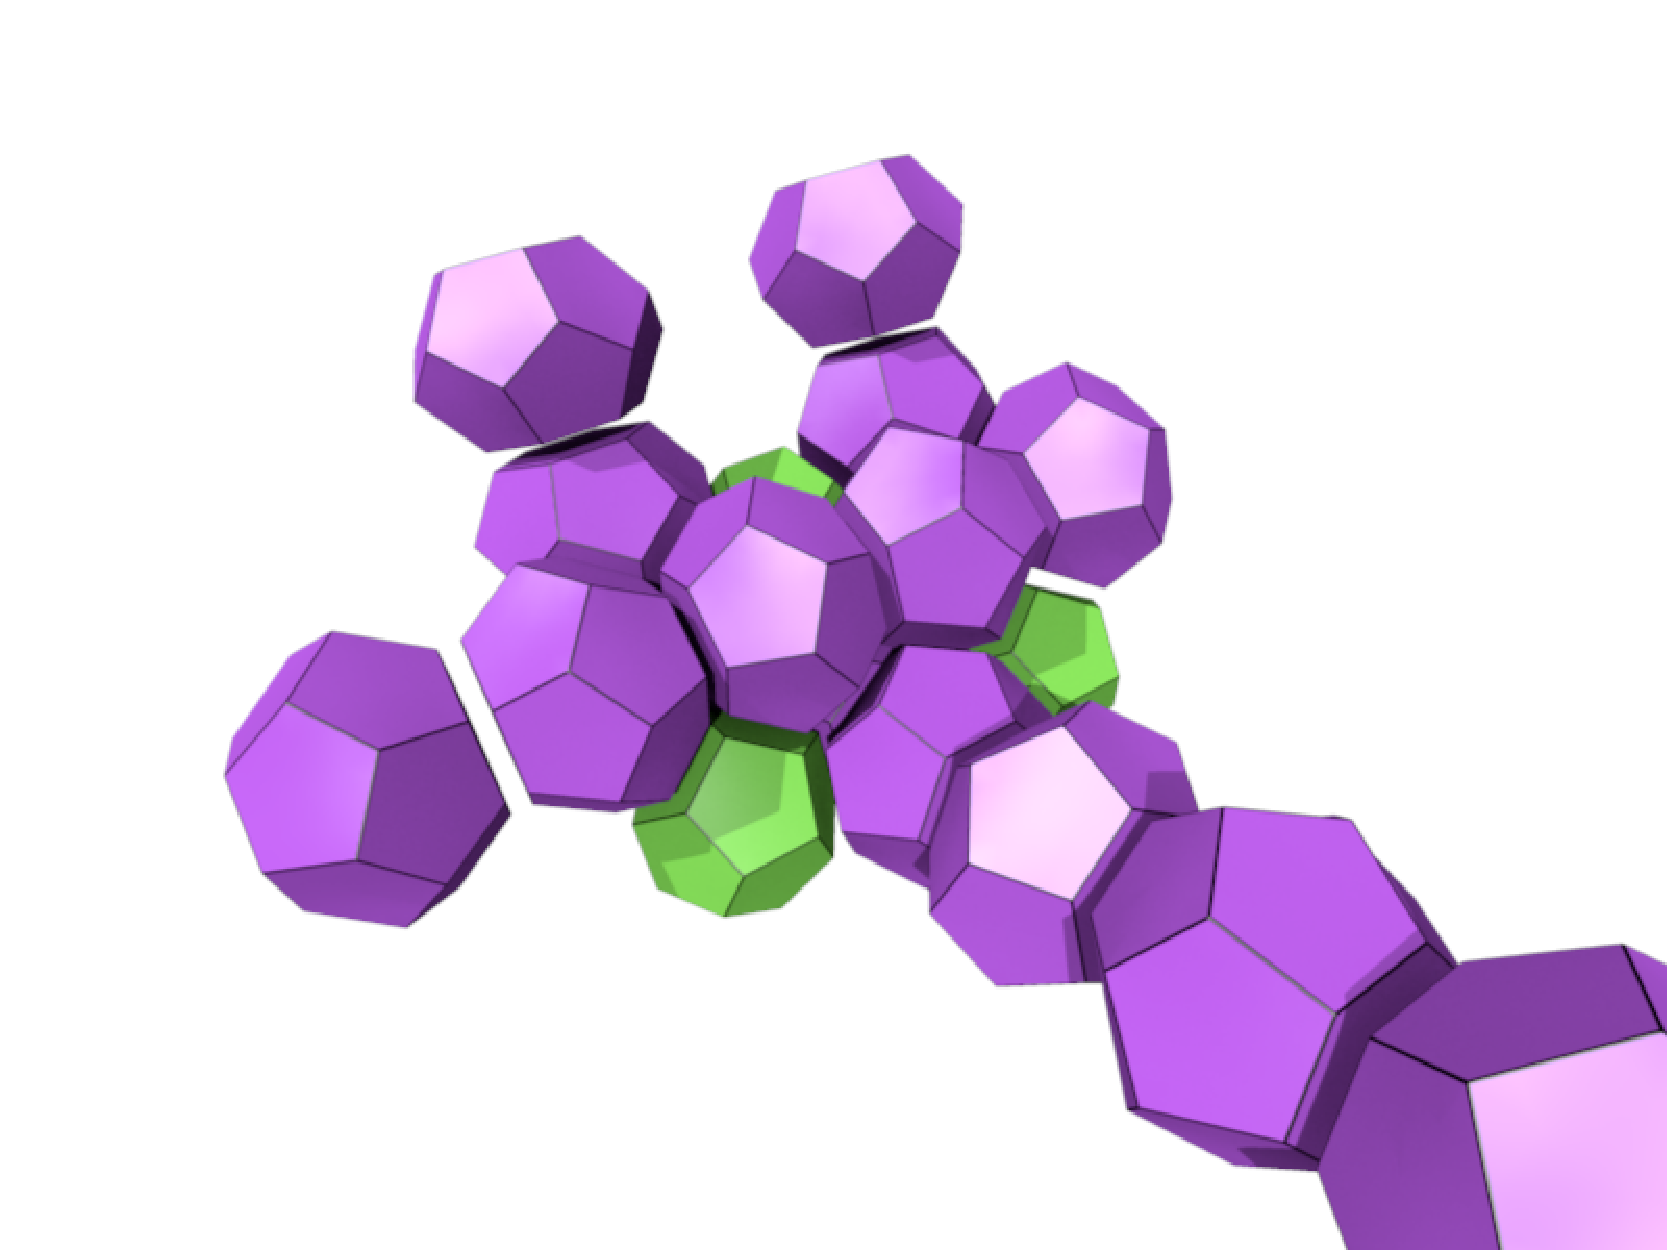
\includegraphics{SpaceFullPicture/A15_1bis.pdf}}\par
\end{center}
Uniquely determined by fractional composition.
}


\frame{
  \frametitle{One structure $(3,2,2,0)$}

\begin{center}
\resizebox{9.5cm}{!}{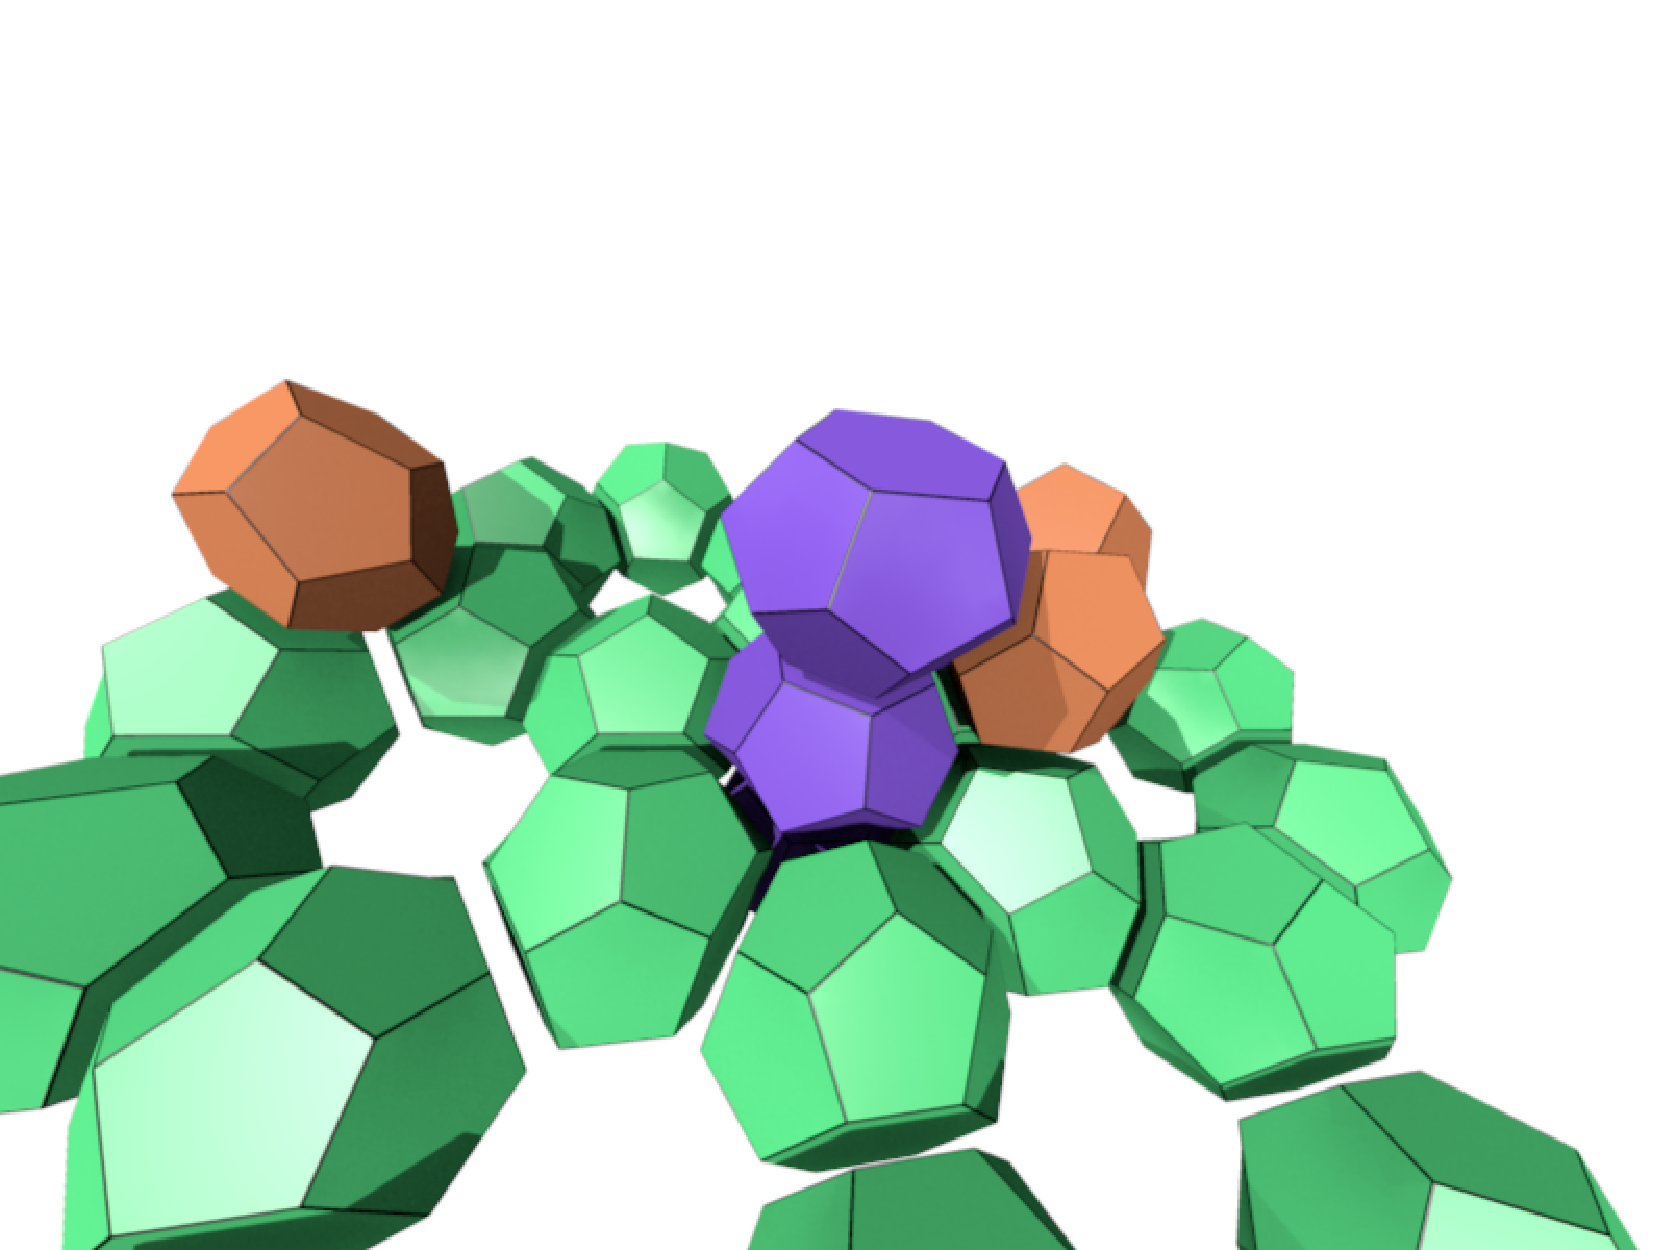
\includegraphics{SpaceFullPicture/Struct7.pdf}}\par
\end{center}
This structure is named $Z$ and is not determined by its fraction.
}
\frame{
  \frametitle{Other structure $(3,2,2,0)$}

\begin{center}
\resizebox{9.5cm}{!}{\includegraphics{SpaceFullPicture/Struct14_63.pdf}}\par
\end{center}
}
\frame{
  \frametitle{Other structure $(3,2,2,0)$}

\begin{center}
\resizebox{9.5cm}{!}{\includegraphics{SpaceFullPicture/Struct14_65.pdf}}\par
\end{center}
}
\frame{
  \frametitle{Other structure $(3,2,2,0)$}

\begin{center}
\resizebox{9.5cm}{!}{\includegraphics{SpaceFullPicture/Struct14_78.pdf}}\par
\end{center}
}







\frame{
  \frametitle{One structure $(3,3,0,1)$}

\begin{center}
\resizebox{9.5cm}{!}{\includegraphics{SpaceFullPicture/Struct14_52.pdf}}\par
\end{center}
}
\frame{
  \frametitle{One structure $(3,3,0,1)$}
\begin{center}
\resizebox{9.5cm}{!}{\includegraphics{SpaceFullPicture/Struct14_54.pdf}}\par
\end{center}
}
\frame{
  \frametitle{One structure $(3,3,0,1)$}

\begin{center}
\resizebox{9.5cm}{!}{\includegraphics{SpaceFullPicture/Struct14_74.pdf}}\par
\end{center}
}






\frame{
  \frametitle{One structure $(2,0,0,1)$}

\begin{center}
\resizebox{9.5cm}{!}{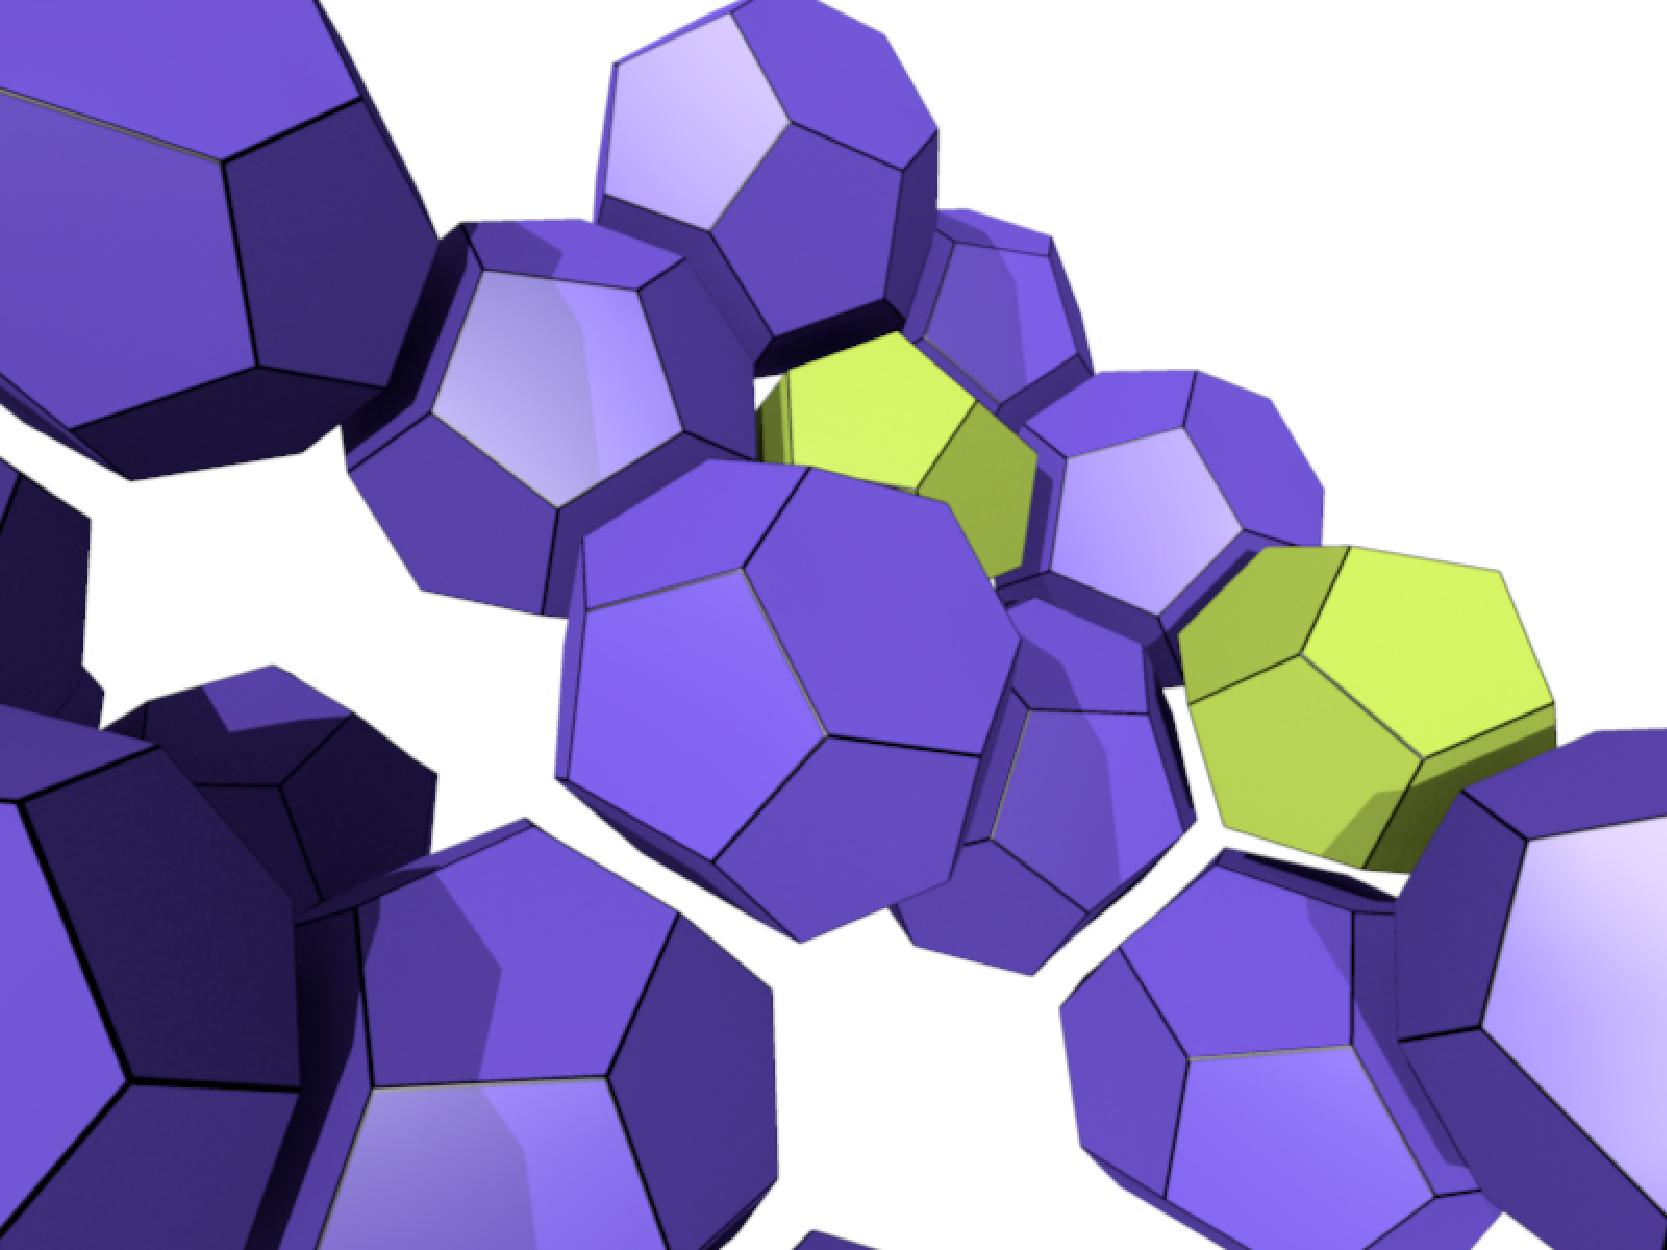
\includegraphics{SpaceFullPicture/Struct1.pdf}}\par
\end{center}
The $28$ maximal cells forms a diamond structure named $C_{15}$.
There is a continuum of such structures.
}



\frame{
  \frametitle{One structure $(7,2,2,2)$}

\begin{center}
\resizebox{9.5cm}{!}{\includegraphics{SpaceFullPicture/Struct39.pdf}}\par
\end{center}
It is a mix of $C_{15}$ and $A_{15}$ in layers.
}



\frame{
  \frametitle{One structure $(7,2,2,2)$}

\begin{center}
\resizebox{9.5cm}{!}{\includegraphics{SpaceFullPicture/Struct41.pdf}}\par
\end{center}
It is a mix of $Z$ and $C_{15}$ in layers.
}





\frame{
  \frametitle{One structure $(5,2,2,1)$}

\begin{center}
\resizebox{9.5cm}{!}{\includegraphics{SpaceFullPicture/Struct18.pdf}}\par
\end{center}
%It is a mix of $Z$ and $C_{15}$ in layers.
}





\frame{
  \frametitle{One structure $(4,5,2,0)$}

\begin{center}
\resizebox{9.5cm}{!}{\includegraphics{SpaceFullPicture/Struct19.pdf}}\par
\end{center}
It is a mix of $Z$ and $A_{15}$ in layers.
}



\frame{
  \frametitle{A counterexample}

\begin{center}
\resizebox{9.5cm}{!}{\includegraphics{SpaceFullPicture/Struct14_17.pdf}}\par
\end{center}
The smallest structure with $-x_{20}+\frac{x_{24}}{3}+\frac{7}{6}x_{26}+2x_{28}\not= 0$
}








\frame{

\vspace{1.5cm}
\begin{center}
{\Huge \textcolor{red}{T}\textcolor{blue}{H}\textcolor{green}{A}\textcolor{blue}{N}\textcolor{red}{K}}\\[1cm]
{\Huge \textcolor{red}{Y}\textcolor{blue}{O}\textcolor{red}{U}}
%\epsfig{file=plit-gal10.eps, height=5.5cm}
\end{center}
}


\end{document}
